\documentclass[14pt]{beamer}

\usepackage{listings}
\lstloadlanguages{python}

\usepackage{color}
\usepackage{tikz}


\mode<presentation>
{
\usetheme{AlpesLasers}
\setbeamercovered{transparent}
  %\setbeamertemplate{footline}[frame number] 
  %\setbeamertemplate{navigation symbols}{ 
  %\hskip 0.3cm
  %\insertframenumber / \inserttotalframenumber  % <<< frame #
  %\insertpagenumber / \insertpresentationendpage % <<< page #
%} 
}

% font definitions, try \usepackage{ae} instead of the following
% three lines if you don't like this look
\usepackage{mathptmx}
\usepackage[scaled=.90]{helvet}
\usepackage{courier}
\usepackage[T1]{fontenc}
\usepackage[english]{babel}
\usepackage[latin1]{inputenc}
\title{Infrared receptors in pyrophilous\\ ("fire loving") insects as model for new un-cooled infrared sensors (2011)}
\subtitle{A Golay Cell overview}
\author{St\'ephane Poss}
\date{\today}
% This is only inserted into the PDF information catalog. Can be left
% out.
\subject{ALDIRAC}


\begin{document}
\begin{frame}[plain]
\titlepage
\end{frame}

\section{Introduction}

\begin{frame}
\tableofcontents
\end{frame}

\section{The authors}
\begin{frame}
\frametitle{The authors}
\begin{enumerate}
\item David Klocke
\item Anke Schmitz
\item Helmut Soltner
\item Herbert Bousack
\item Helmut Schmitz*
\end{enumerate}
Institute of zoology, University of Bonn,\\
Forschungszentrum J\"ulich GmbH, Zentralabteilung Technologie,\\
Forschungszentrum J\"ulich GmbH, Peter Gr\"unberg Institut
\end{frame}

\section{A bit of biology}
\begin{frame}
\frametitle{Fire loving beetles?}
\begin{quote}
Fire loving (pyrophilous) insects depend on forest fires for their reproduction.
\end{quote}
\begin{columns}
\column{0.49\textwidth}
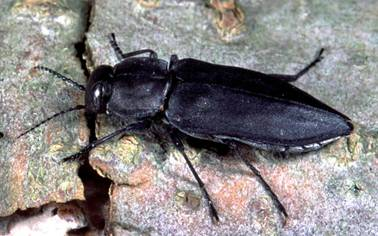
\includegraphics[width=\textwidth]{kaefer_03.jpg}
\column{0.6\textwidth}
\begin{quote}
[...] these insects have special sensors for smoke and infrared radiation.
\end{quote}
\end{columns}
Distribution: more or less everywhere
\end{frame}

\begin{frame}
\frametitle{How/why}
\begin{itemize}
\item \emph{Often stay on the stem of trees close to burning or glowing wood or hot ashes}
\item They \emph{try to copulate vigorously}
\item Females \emph{deposit the eggs under the bark of burnt trees}
\item The larvae can \emph{only develop in the wood of burnt trees}
\end{itemize}
Fire detection is obviously an important requirement for the survival of the pyrophilous insects
\end{frame}

\begin{frame}
\frametitle{Requirements/solution}
\begin{itemize}
\item Must be able to detect heat from a distances as large as possible
\item Ability to avoid ``hot'' spots $>60^oC$ (dangerous)
\end{itemize}
\pause
Solution:\\
\begin{quote}
\alert{These insects feature so-called photomechanic IR receptors} which might serve well as models for the technical design of un-cooled IR receptors.
\end{quote}
\end{frame}

\begin{frame}
\frametitle{Mechanoreceptors}
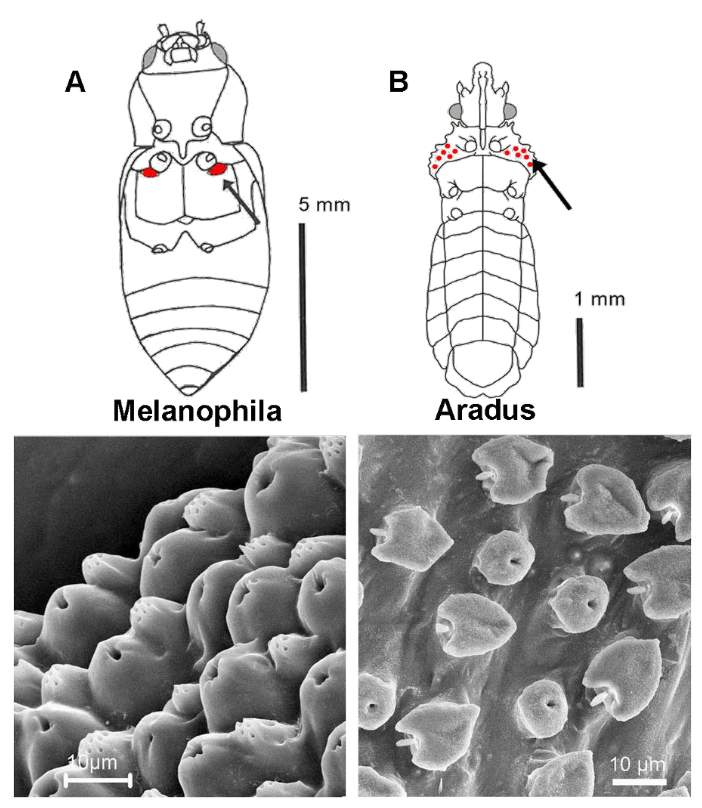
\includegraphics[width=7cm]{beetles_sensors.png}
\end{frame}
\begin{frame}
\frametitle{Mechanoreceptors}
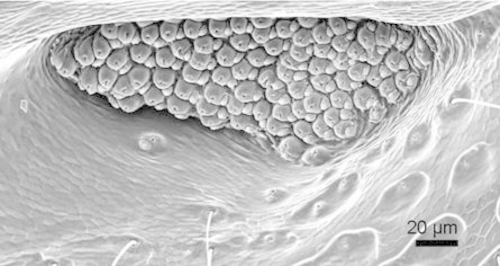
\includegraphics[width=8cm]{6974e8e62f.jpg}\\
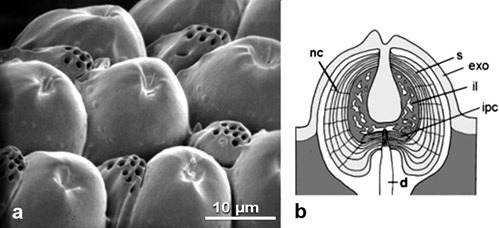
\includegraphics[width=8cm]{IR_sensor_abb_3_02.jpg}
\end{frame}
\begin{frame}
\frametitle{Mechanoreceptors}
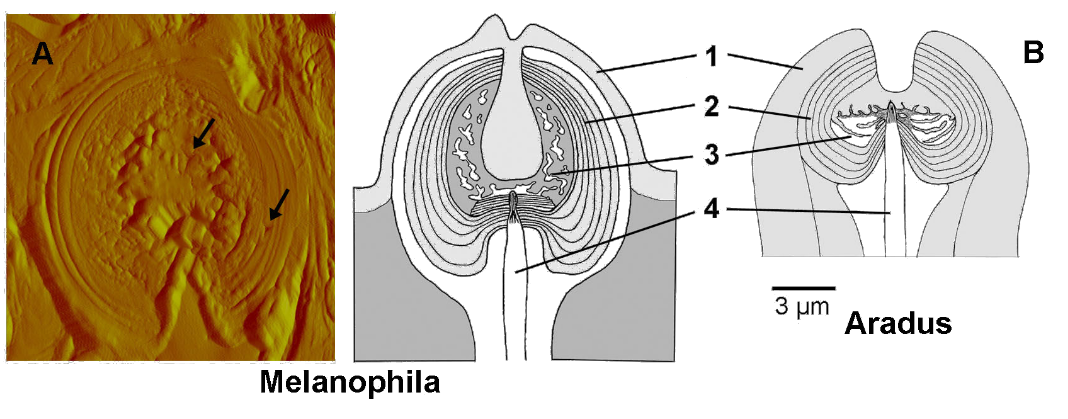
\includegraphics[width=10cm]{mechanoreceptor.png}
\begin{enumerate}
\item outer exocuticle (hard)
\item exocuticular shell of the inner sphere (hard)
\item microfluidic core
\item tip of the mechanosensory dendrite
\end{enumerate}
\end{frame}


\begin{frame}
\frametitle{Working principles}
\begin{quote}
Most probably, IR radiation absorbed by the proteins, the chitin fibres, and the water of the sensillum heats up the sphere, which immediately causes \alert{thermal expansion} especially of the liquid inside the microfluidic core.
\end{quote}
\begin{quote}
[...] the only \alert{compliant structure} in the sphere is the \alert{membrane} of the tip of the \alert{mechanosensitive dendrite.}
\end{quote}
\end{frame}

\section{Golay cell}

\begin{frame}
\frametitle{Pneumatic detector model}
Marcel J.~E.~Golay, review of Scientific Instruments 18, 347(\alert{1947})
\begin{itemize}
\item model pneumatic circuits like electric ones
%\begin{itemize}
%\item Physics knowledge is evolving rapidly
%\item Need to find new detection tools
%\end{itemize}
\item most of it is forgotten now
\begin{itemize}
\item who has heard of pneumatic capacitance?
\end{itemize}
\item most important part: Golay Cell development
\end{itemize}
Start principle: energy measurement is about observing the geometrical displacement of something
\end{frame}

\begin{frame}
\frametitle{Considerations, concepts}
\begin{itemize}
%\item thermal capacity: $\frac{C}{T}$
%\item thermal resistance: 1/rate at which a differential heat flow between the background and the black body will take place, due to sudden change of temperature
\item \alert{no substance is known to act simultaneously as a black body and as sensitive thermometer having a small calorific inertia}
\item Chose either:
\begin{itemize}
\item electrical translating: thermopile, bolometer
\item heat received passes in a gas of a cell closed by an optical deflecting membrane: opto-acoustical detectors
\end{itemize}

\end{itemize}

\end{frame}
\begin{frame}
\frametitle{Considerations, concepts}
\begin{itemize}
\item heat conductivity of the gas: heat leakance = noise
\item pneumatic ohm: pneumatic resitance across which a pressure of 1 bar is developed by a gaseous flow of one $\mathrm{cm}^3\mathrm{s}^{-1}$.
\item pneumatic farad: incremental pressure of one bar causes the admission of $1 \mathrm{cm}^3$ of gas 
\end{itemize}
\end{frame}
\begin{frame}
\frametitle{A look into the Golay Cell}
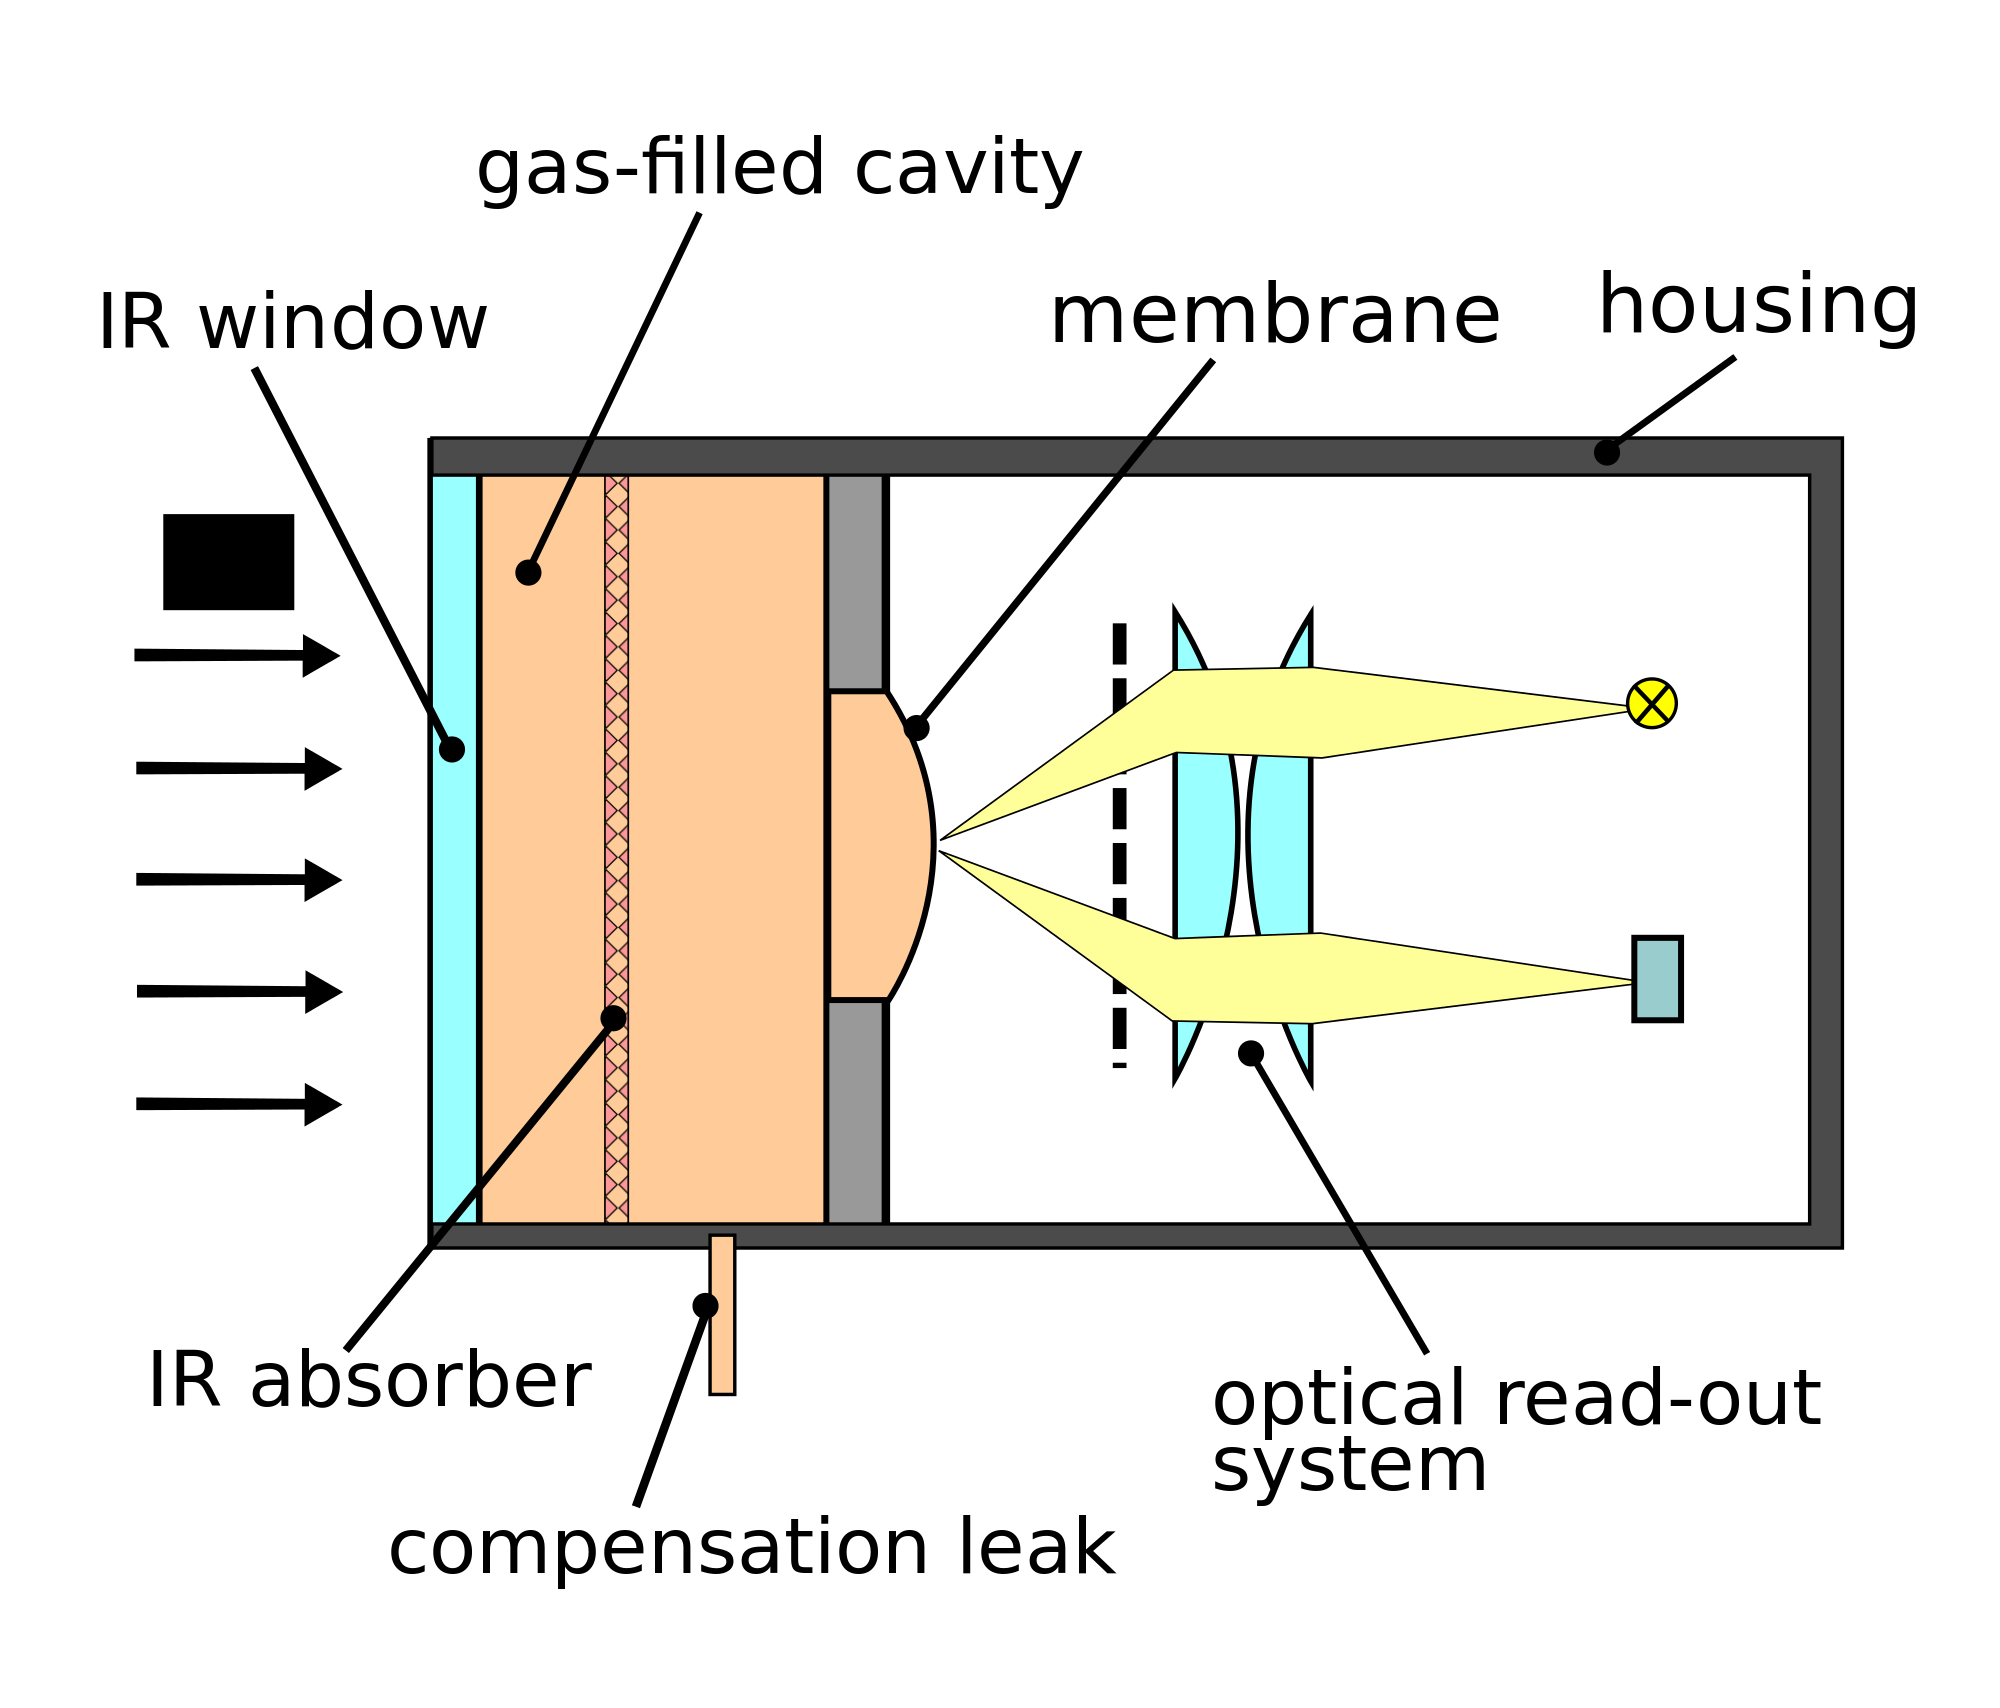
\includegraphics[width=9cm]{2000px-Golay_Cell_Schematic.png}
\end{frame}


\section{Back to insects}
\begin{frame}
\frametitle{Modelling the mechanoreceptor}
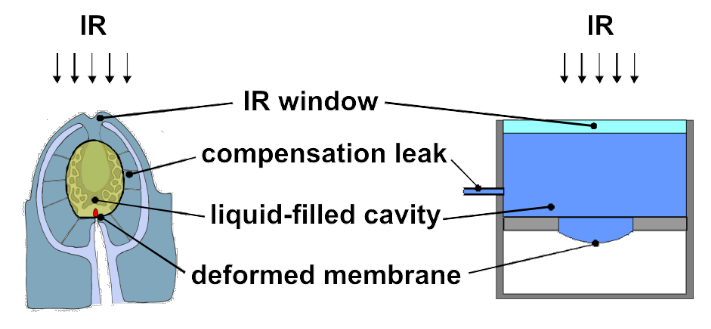
\includegraphics[width=10cm]{themodel.png}
\end{frame}

\begin{frame}
\frametitle{A bit of math}
\begin{eqnarray}
\Delta P &=& \frac{\beta \Delta T_{mean}}{1+\Omega}\\
\Delta T_{mean} &=& \frac{\int_0^{H_c} \Delta T(z) dz}{H_c}\\
\Omega &=& \frac{R^4(1-v^2)}{16\cdot E \cdot t_p^3 \cdot H_c \cdot\kappa}\\
\kappa &=& -(1/V)(\delta V/\delta P)_T\\
y_{max} &=& \frac{3\beta\kappa \Omega \Delta T_{mean} H_c}{1+\Omega}
\end{eqnarray}
$\kappa$ is medium compressibility: for water $=4.5\times 10^{-10} \mathrm{Pa}^{-1}$


\end{frame}

\begin{frame}
\frametitle{Comparing media}
\begin{columns}
\column{0.6\textwidth}
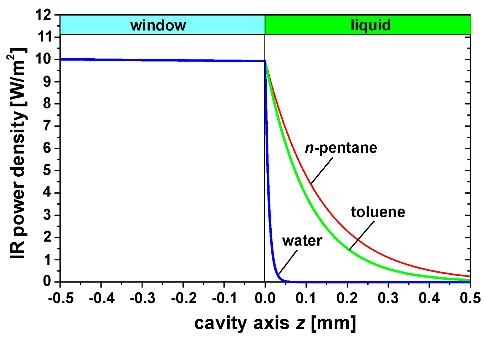
\includegraphics[width=\textwidth]{IRPowerDensity.png}\\
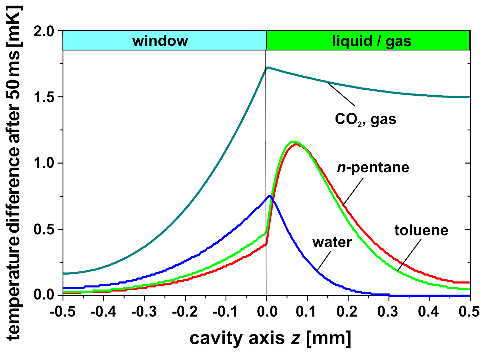
\includegraphics[width=\textwidth]{TemperatureDist.png}
\column{0.6\textwidth}
$10\mathrm{mW}/\mathrm{m}^2, \mathrm{after}~0.5s$:
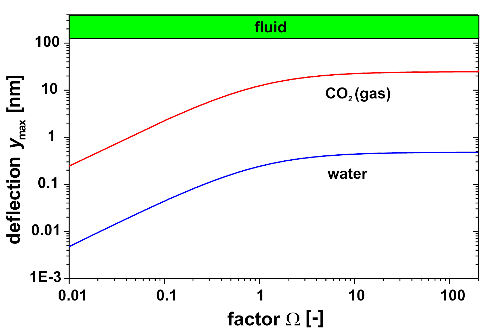
\includegraphics[width=\textwidth]{maxdeflexion.png}\\
Max deflection for \\water: 0.2nm, gas: 12nm\\
\end{columns}
\end{frame}
\begin{frame}
\frametitle{Readout}
\begin{quote}
The calculated deformation [...] for water as liquid and the deformation of the [...] dendrite [...] have same magnitude. [...] deformations of the tip of the dendrite of only 0.1nm [...] yield a receptor potential. 
\end{quote}
Proposed readout: interferometry, tunneling contacts or capacitive position sensor with nm resolution.
\end{frame}

\section{A working prototype}
\begin{frame}
\frametitle{A built prototype}
From the Center of advanced european studies and research:\\
~\\
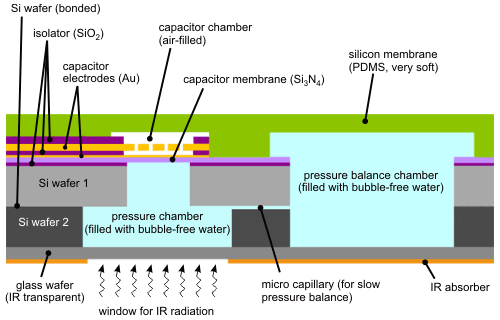
\includegraphics[width=8cm]{IR_sensor_abb_4_02.png}
\end{frame}
\begin{frame}
\frametitle{A built prototype}
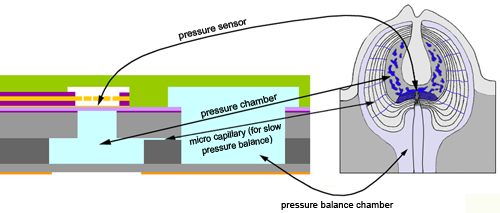
\includegraphics[width=10cm]{IR_sensor_abb_5_02.png}
\end{frame}

\section{Other detector for FIR}
\begin{frame}
\frametitle{Comparing Golay cells and pyroelectric detectors}
Pyroelectric detectors: ferroelectric crystal (e.g. LiTaO3), instantaneous polarization is a funtion of the rate of temperature change in crystal

\end{frame}

\begin{frame}
\frametitle{Comparing}
From Spectrum Detector Inc.:\\

\begin{columns}
\column{0.6\textwidth}
Golay Cell
\begin{itemize}
\item very sensitive (sub nW)
\item broad spectral response
\item well characterized
\item low power only (10$\mu W$ max)
\item very fragile
\item expensive (\$10K-\$15K)
\end{itemize}
\column{0.6\textwidth}
Pyroelectric
\begin{itemize}
\item sensitive (nW)
\item broad spectral response
\item fast
\item up to 10mW
\item cheap (\$450 to \$2000)
\item lower efficiency
\item not well charaterized
\item microphonic response requires care
\end{itemize}
\end{columns}
\end{frame}

\section{Conclusion}
\begin{frame}
\frametitle{Conclusion}
\begin{itemize}
\item Insects possess very sensitive mechanoreceptor
\item Difficult to achieve for a technical sensor
\item Need a very precise readout system, 1nm resolution
\item prototype sensor was developed at CAESAR
\item Need to optimise the liquide in the cavity, but very hard to build
\end{itemize}
Nature still has a lot to teach us about sensors!
\end{frame}

\appendix

\begin{frame}
\frametitle{Other natural IR detectors}
\begin{columns}
\column{0.6\textwidth}
\begin{itemize}
\item Pit viper 
\item Red-bodied Swallowtails (butterfly)
\item "kissing bug" or "barber bug" (no pic, disgusting)
\item vampire bat
\item common carp?
\item other fish?
\end{itemize}
\column{0.45\textwidth}
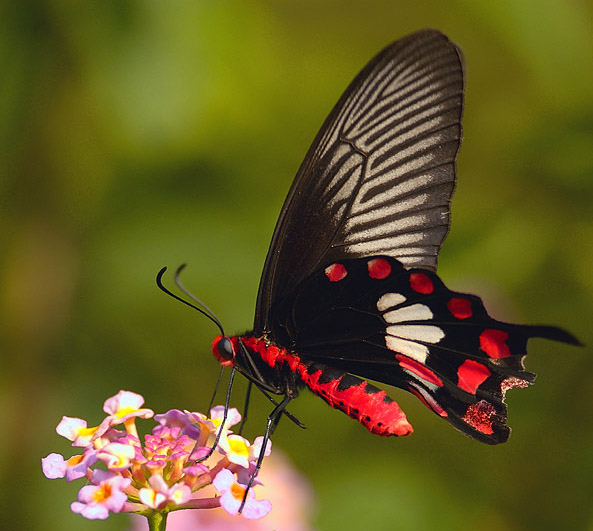
\includegraphics[width=\textwidth]{2005-common-rose.jpg}
\end{columns}
\end{frame}

%{
%\usebackgroundtemplate{\includegraphics[width=\paperwidth]{cyborg.jpg}}
%\setbeamertemplate{headline}{\includegraphics[width=\paperwidth]{cyborg.jpg}}
%\begin{frame}
%\vspace{6.cm}Thanks to Samuele, Romain, Tobias, \\Antoine, for useful input. More discussions \\will be needed!
%\end{frame}
%}

\end{document}
